Вторая лабораторная работа заключается в реализации преобразований поворота на основе частного случая углов Эйлера, реализация класса исключений для движка, и написания автотестов. 


\subsection{Определения}

	Определим частный случай поворотов с помощью углов Эйлера -- углы поворота Тейта-Брайана. Для начала введем понятие матрицы поворота в двумерном пространстве.

	Матрицей поворота в двумерном пространстве называется матрица следующего вида:
	\[ R \pares{\alpha} = \begin{pmatrix} \cos{\alpha} & -\sin{\alpha} \\ \sin{\alpha} & \cos{\alpha} \end{pmatrix}. \]
	Данная матрица при применении на любой вектор в правосторонней системе координат совершает поворот представленного вектора <<против часовой стрелке>> на заданный угол $\alpha$. В трехмерном случае такую матрицу можно применить в поворотах относитель трех пар координатных осей: XY, YZ, XZ. Для каждой пары согласно четности перестановки матрицы поворота вокруг соответствующих осей будут иметь следующий вид:
	\[ 
		R_x \pares{\alpha} = 
		\begin{pmatrix} 
			1 & 0 & 0 \\ 
			0 & \cos{\alpha} & -\sin{\alpha} \\ 
			0 & \sin{\alpha} & \cos{\alpha} 
		\end{pmatrix}
	\] 
	\[
		R_y \pares{\beta} = 
		\begin{pmatrix} 
			\cos{\beta} & 0 & \sin{\beta} \\ 
			0 & 1 & 0 \\ 
			-\sin{\beta} & 0 & \cos{\beta}
		\end{pmatrix} 
	\]
	\[ 
		R_z \pares{\gamma} = 
		\begin{pmatrix} 
			\cos{\gamma} & -\sin{\gamma} & 0 \\ 
			\sin{\gamma} & \cos{\gamma} & 0 \\ 
			0 & 0 & 1
		\end{pmatrix}
	\]
	Общее преобразование поворота на углы $\alpha, \beta, \gamma$ вокруг осей $Ox, Oy, Oz$ согласно поворотам Тейта-Брайана будет принимать следующий вид:
	\[ R_{x, y, z} \pares{\alpha, \beta, \gamma} = R_x \pares{\alpha} \cdot R_y \pares{\beta} \cdot R_z \pares{\gamma}. \]

	Также можно ввести обобщение матрицы поворота в $n$-мерном пространстве. 

	\textit{Определение:} Матрицей поворота в плоскости, образованой осями $Ox_i$ и $Ox_j$ называется блочно-диагональная матрица \( \pares{\pares{r_{p, q}^{}}^{\vphantom{1}}}_{p, q = \overline{1, n}} \), на главной диагонали которой лежат единицы, кроме элементов \( r_{i, i} = r_{j, j} = \cos{\alpha} \). В элементах \( r_{i, j} \) и \( r_{j, i} \) будет находиться $\sin{\alpha}$ с точностью до знака согласно перестановке координат. Общий вид:

	\[ R_{i, j}\pares{\alpha} = \begin{pmatrix} 
		\mathbf{I} & \mathbf{0} & \mathbf{0} & \mathbf{0} & \mathbf{0} \\
		\mathbf{0} & \cos{\alpha} & \mathbf{0} & \pares{-1}^{i + j} \sin{\alpha} & \mathbf{0} \\
		\mathbf{0} & \mathbf{0} & \mathbf{I} & \mathbf{0} & \mathbf{0} \\
		\mathbf{0} & \pares{-1}^{i + j + 1} \sin{\alpha} & \mathbf{0} & \cos{\alpha} & \mathbf{0} \\
		\mathbf{0} & \mathbf{0} & \mathbf{0} & \mathbf{0} & \mathbf{I}
	\end{pmatrix} \]
	Для получения такой матрицы, выполняется следующая последовательность действий:
	\begin{enumerate}
		\item \( R_{i, j} = \pares{\pares{r_{p, q}^{}}^{\vphantom{1}}}_{p, q = \overline{1, n}} = I_{n} \);
		\item \( r_{i, i} = r_{j, j} = \cos{\alpha} \);
		\item \( r_{i, j} = - r_{j, i} = \pares{-1}^{i + j} \sin{\alpha} \).
	\end{enumerate}
	В результате будет получена требуемая матрица поворота.


\subsection{Исключения}

	Теперь перейдем к разделу исключений. Для реализации движка желательно реализовать собственные подклассы исключений для различных разделов игрового движка. Это необходимо для более точечной классификации ошибок работы движка. В качестве рекомендации предлагается ввести общий класс исключений (например, \inlinecode{EngineException}), относительно которого создать отдельные подклассы исключений для различных случаев (например, \inlinecode{MatrixException}). Внутри каждого отдельного класса исключений можно задать распространенные тексты ошибок в виде полей или методов класса:

	\begin{figure}[H]
\begin{lstlisting}[caption=<<Пример (Python)>>]
class EngineException(Exception):
	pass

class MatrixException(EngineException):
	MATRIX_UNKNOWN_OPERATION = "This operation isn't defined for matrix"

	@staticmethod
	def MATRIX_WRONG_SIZES(n1: int, m1: int, n2: int, m2: int) -> str:
		return f"Wrong sizes: {n1}x{m1} and {n2}x{m2}"

class VectorException(EngineException):
	VECTOR_UNKNOWN_OPERATION = "This operation isn't defined for vector"
\end{lstlisting}
	\end{figure}

	Также возможен и другой вариант. Для каждого варианта исключения можно оформить свой класс (с сообщением, которое затем вызывать):
	\begin{figure}[H]
\begin{lstlisting}[caption=<<Пример (Python)>>]
class EngineException(Exception):
	pass

class MatrixWrongSizeException(EngineException):
	@staticmethod
	def MESSAGE(n1: int, m1: int, n2: int, m2: int) -> str:
		return f"Wrong sizes: {n1}x{m1} and {n2}x{m2}"

class MatrixIncorrectOperationException(EngineException):
	MESSAGE = "Incorrect operation"
\end{lstlisting}
	\end{figure}


\subsection{Модульное тестирование}

	Теперь по поводу модульного тестирования. Такое тестрование необходимо для больших проектов для проверки модулей на работоспособность при внесении в них каких-либо изменений. В нашем движке необходимо реализовать тесты на все реализуемые модули. Для упрощения написания тестов можно воспользоваться уже готовыми фреймворками, которые, к примеру, могут быть интегрированы в среду разработки.

	Рассмотрим некоторые примеры фреймворков:
	\begin{enumerate}
		\item <<C++>> -- <<GTest>>, <<Catch2>>, и др.;
		\item <<Python>> -- <<pytest>>;
		\item <<Java>> -- <<JUnit>>;
		\item <<C\#>> -- <<MS Test>>;
		\item <<Rust>> -- встроенная утилита <<cargo test>>
	\end{enumerate}

	Обсудим вопрос наименований и самой логики тестирования. Как было сказано ранее, тестирование должно проводиться для каждого модуля индивидуально, соотвественно название модуля тестирования можно писать через название с подписью <<Tests>>: \inlinecode{LowLevelClasses.Tests}. Для каждого модуля создаем классы, содержащие говорящие названия того, что тестируется, и подписью <<Tests>>: \inlinecode{MatrixOperationsTests}, \inlinecode{VectorOperationsTests}. Внутри классов задаем методы с названием, в котором отображается суть теста. Также стоит придерживаться единого метода написания тестов. Более простым и очевидным методом считается метод <<Arrange -- Act -- Assert>>, в котором код каждого теста разделяется на три основные части по следующему принципу:
	\begin{enumerate}
		\item <<Arrange>> -- Настройка тестового окружения, введение переменных, с которыми будем работать;
		\item <<Act>> -- Выполнение действия, которое необходимо протестировать с заданными переменными;
		\item <<Assert>> -- Проверка того, что выполненное действие является корректным.
	\end{enumerate} 

	\begin{figure}[H]
\begin{lstlisting}[caption=<<Пример (Python)>>]
#File: LowLevelOperations.Tests
class MatrixOperationsTests:
	def MatrixAddition(self):
		#Arrange
		matrix1 = Matrix([[1, -1], [-1, 1]])
		matrix2 = Matrix([[0, 1], [1, 0]])
		matrix3 = Matrix([[1, 0], [0, 1]])

		#Act
		result = matrix1 + matrix2

		#Assert
		assert result == matrix3
\end{lstlisting}
	\end{figure}

	Также к рекомендациям можно отнести выделенное тестирование -- тестируем ровно одну операцию за один раз. Никаких множественных \inlinecode{assert} быть не должно, так как могут возникать ошибки при тестировании. Самый простой вариант -- когда тест не прошел на одном \inlinecode{assert}, то система тестирования в большинстве случаев проигнорирует дальнейшее выполнение теста, в силу чего автор возможно не узнает о наличии ошибок в дальнейших тестах. Необходимо принять за правило: один тест содержит ровно один \inlinecode{assert}.


\subsection{Документация}

	Для проекта рекомендуется ввести документацию. Она включает в себя детальное описание реализуемых модулей с примерами применения тех или иных частей проекта в реализации. В качестве примера можно привести любую документацию к языкам программирования.

	Реализация документации производится на странице Wiki пользовательского репозитория проекта на сервисах <<GitHub>> (\textit{только в публичных репозиториях}) или <<GitLab>>. Страницы распределяются по классам. Если классы содержат не так много документируемой информации, при этом являются смежными классами, то их можно объединить на одной странице. Документация предпочтительно может быть написана на английском языке, но и вариант с русским языком также возможен. В дополнение, код так же должен быть задокументирован в самом исходном коде каждого модуля. Реализация документирования внутри исходного кода является индивидуальной для каждого языка.

	Страница должна содержать следующую информацию:
	\begin{enumerate}
		\item Название класса (или обобщение названия для смежного набора классов);
		\item Краткая характеристика класса/классов -- информация о странице, о том, что описывается, и другое;
		\item Информация о том, как импортируется модуль с данными классами;
		\item Информация о классе/классах -- инициализация, список полей, список методов (в логическом порядке), список перегруженных операторов. Для каждого поля, метода и оператора прописать полагаемые типы данных на входе, и ожидаемый тип данных на выходе;
		\item Примеры использования с выводом (в виде комментария).
	\end{enumerate}

\pagebreak
\vspace*{-90pt}
	\begin{figure}[H]
		\begin{lstlisting}[language=XML, caption=Краткий пример страницы <<Matrix>> на языке <<Markdown>>]
# Matrix
This page contains information about class `Matrix`. Matricies are basic algebraic objects, used in math...

## Initialization:
Possible variants for initialization:
- `Matrix(n: int, m: int)` &mdash; creates zero matrix with `n` rows and `m` columns;
- `Matrix(elements: list[list[any]])` &mdash; creates matrix with default values (about values [here](about:blank));
...

## Attributes:
- `n: int`, `m: int` &mdash; count of matrix rows and columns;
- `data: list[list[any]]` &mdash; matrix data;
...

## Methods:
- `set_value(i: int, j: int, value: any) -> None` &mdash; method sets value for `i` row and `j` column;
- `determinant() -> float` &mdash; method called for square matrix, which return its determinant;
- `Matrix.identity(n: int) -> Matrix` &mdash; static method which returns square identity matrix with size `n`;
...

## Overloaded:
- `Matrix + Matrix -> Matrix` &mdash; matrix addition operator;
- `Matrix * Matrix | int | float -> Matrix` &mdash; matrix multiplication operator;
...

---

# Examples
### Example 1: 
Matrix initialization, multiplication and determinant usage
```Python
matrix1 = Matrix([[1, 0, 1], [0, 1, 2]])
matrix2 = Matrix([[-1, 2], [0, 1], [2, -3]])

matrix3 = matrix1*matrix2 # Matrix([[1, -1], [4, -5]])
matrix4 = matrix2*matrix3 # Matrix([[-1, 2, 3], [0, 1, 2], [2, -3, -4]])

print(matrix3.determinant(), matrix4.determinant())
# Result: -1, 0
```

### Example 2: 
Something else...
		\end{lstlisting}
	\end{figure}

	\begin{figure}[H]
		\centering
		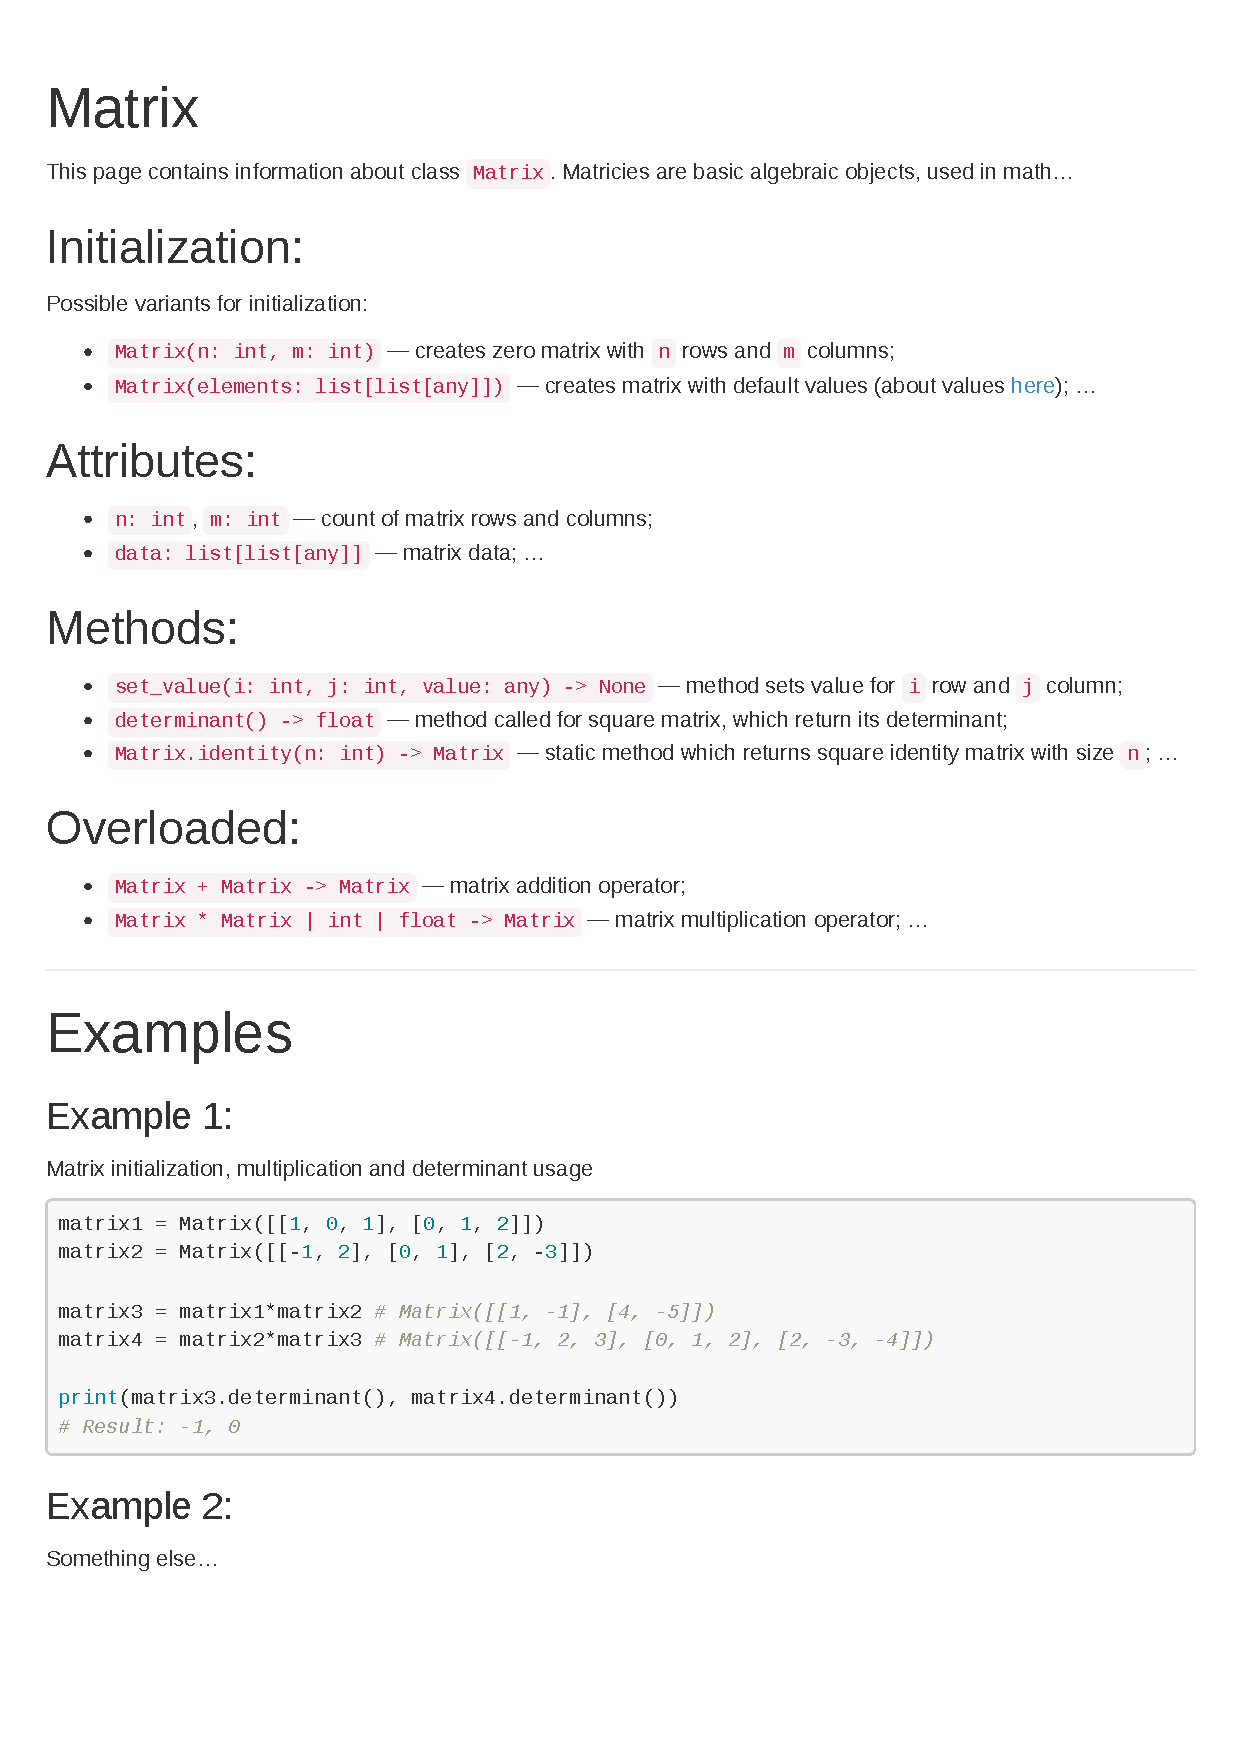
\includegraphics[height=0.9\textheight]{additional/page.pdf}
		\caption{Визуальный пример страницы <<Matrix>> на языке <<Markdown>>}
	\end{figure}

	Также, документацию можно оформить отдельными файлами в заданной папке документации, описывающей индивидуально каждую страницу.


\subsection{Этапы реализации}

	Зафиксируем представленную информацию:
	\begin{enumerate}
		\item Разделим весь проект на модули. Классы, отвечающие за математическое составляющее движка необходимо вынести в отдельный файл, так же другие части движка, такие как исключения нужно вынести отдельно;
		\item В класс матриц введем операции поворота относительно осей с помощью преобразований углов Тейта-Брайана;
		\item Введем собственный класс исключений на основе базового класса, который будет содержать необходимые поля и методы для реализации выводов именованых исключений в модулях;
		\item Проведем модульное тестирование для уже готовых классов. Тестирование должно быть структурировано таким образом, чтобы оно затрагивало все созданные операции в модуле. Важно обратить внимание на наименование файлов, классов и методов в тесте;
		\item Введем документацию, содержащую информацию о классах, их полях и методах, зависимостях. В документации реализуем список изменений.

	\end{enumerate}

	В дальнейшем сдача лабораторных работ будет производиться по следующим критериям:
	\begin{enumerate}
		\item Список изменений с последней сдаваемой версии проекта;
		\item Документация проделанной работы с примерами;
		\item Написанные тесты для тех частей проекта, в котором произведены изменения.
	\end{enumerate}


\subsection{Класс Matrix}
	\noindentВ дополнению к классу матриц добавить возможность генерации матрицы поворота.

	\noindent Реализуемые методы:
	\begin{enumerate}
		\item \inlinecode{Matrix.get_rotation_matrix(inds: (int, int), angle: float, n: int) -> Matrix} -- статический метод, возвращающий матрицу поворота в заданной плоскости (по индексам) на заданный угол в пространстве заданной размерности;
		\item \inlinecode{Matrix.get_teit_bryan_matrix(angles: (float, float, float)) -> Matrix} -- статический метод, возвращающий матрицу поворота в $3$-мерном пространстве с помощью преобразования Тейта-Брайана на заданные $3$ угла вокруг осей.
	\end{enumerate}
